\chapter{Related Work}
\label{chap:Related Work}

In the following chapter we lay the foundation for the research conducated in this thesis. We start off with an introduction of the topic of urban heat island (UHI) detection, which is one of the motivating factors behind this work. UHI research is part of the discipline of modern climatology and relies on many different sub-disciplines like meteorology, thermal dynamics, geology and many more.
After discussing traditional ways to detect UHIs, such as using remote satellite data, we discuss newer approaches, especially in the context of smart cities, that focus on collecting air temperatures in urban environments. Measuring data in the urban environment comes with many challenges~\cite{oke2006guideline}, that can lead to missing or wrong observations for given places.
In order to improve data availibility in the urban climate context we compare traditional interpolation techniques based on (geo-)statistics with more recent machine-learning based approaches, that could be used in this highly complex urban setting. This interpolated data could be used to improve interpolation or prediction models and give additional insights into the influences of urban environments, f.e. in the context of UHIs and their detection and analysis.
Finally, in order to compare traditional geostatistical models with ML-based models, we need comprehensive data-sets of urban climate data. An overview of available data sources is given in section \ref{sec: access to data sets} together with an introduction to the OpenData movement.

\section{Urban Heat Islands (UHI)}

UHIs have been the center of a lot of attention for quite some time in the scientific community. As early as 1833, with the research of Luke Howard in London which observed higher temperatures inside London than in surrounding areas~\cite{howard1833climate}, UHIs have seen a steadily increase in scientific contributions. The term \textit{Urban Heat Island} was first introduced in the 1940s~\cite{balchin1947micro}. The recording and investigation of UHIs has seen mayor steps since the begin of modern climatology, also known as the Sundborg's era beginning with Sundborg's 1951 classic heat island study of Uppsala~\cite{sundborg1951climatological}. UHIs occur in many cities around the globe~\cite{peng2012surface} in different climatic zones, during different times of day and in different intensities.\\

\subsubsection{Shared UHI Challenges}

Some shared challenges are: 1. Define what \textit{urban} means in the context of UHIs~\cite{stewart2009newly}. The term urban is widely used to identify areas that are more densly populated than the surrounding rural areas. Having this distinction between urban and rural~\cite{lowry1977empirical} helped researchers to better define the UHI magnitude (cite), but this simple distinction also lead to problems~\cite{stewart2011systematic}. The problem lies in the fact that there is no clear border between urban and rural areas, but a fluent transition. Especially for larger metropolitan areas, like Tokyo, the urban area could span 10s to 100s of kilometers, making the collection of reference rural temperatures hard. The reference rural temperature has a direct influence on the UHI magnitude, which is `the most widely recognized indicator of city climate modification in the encironmental sciences'~\cite{stewart2009newly}. As a solution, different classification into local climate zones were proposed~\cite{stewart2012local, stewart2009newly}, that classify areas based on surface roughness, building densities, building heights etc. 2. Measuring the influence of other local urban or meterological phenomena on the temperatures collected. The urban climate is extremly complex, due to many different influences, such as antropological energy,... (cite, todo find the influence factors). Additionally, the urban climate is also influenced by surrounding regional/meso-scale climate phenomena such as storms, valleys, mountains, large waterbodies, costlines and more (cite).

\subsection{UHI Classification}

UHIs can be classified in many different ways. Typically, there is a horizontal classification, defining the superficial extension of the UHI from micro-, to local- to meso-scale, and a vertical classification, defining in which vertical layer of the urban area the heat island is observed. To better understand these scales and the anatomy of the planitory/urban boundary layer, figures \ref{fig:mesoscale boundary layer} to \ref{fig:microscale boundary layer} show a detailed view of the meso-, local- and micro-scale of the urban climate, as illustrated by Oke 2006~\cite{oke2006guideline}.

\begin{figure}[h]
    \centering
    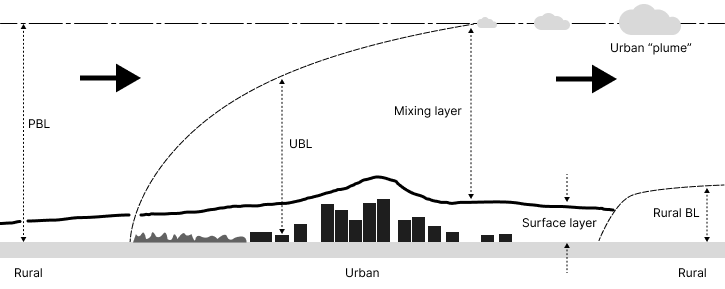
\includegraphics[width=\textwidth]{images/Mesoscale Boundary Layer.png}
    \caption{Mesoscale view of the urban climate, redrawn from~\cite{oke2006guideline}}
    \label{fig:mesoscale boundary layer}
\end{figure}

The mesoscale, as depicted in fig. \ref{fig:mesoscale boundary layer}, spans the whole urban environment of a city, typically tens of kilometres. There are several boundary layers, that comprise different scales. The planetary boundary layer (PBL)~\cite{wyngaard1985structure} is the lowest layer of the Earth's atmosphere and spans from the surface to a height of several hundred meters up to several kilometers. It is characterised by the turbulent mixing of air, forming wind currents, that are mayorly influenced by the underlying surface.

\begin{figure}[h]
    \centering
    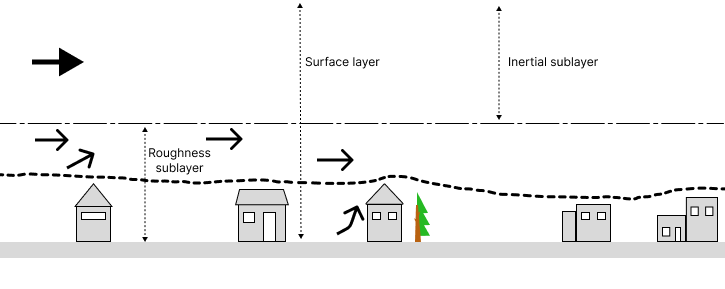
\includegraphics[width=\textwidth]{images/Localscale Boundary Layer.png}
    \caption{Localscale view of the urban climate, redrawn from~\cite{oke2006guideline}, (Todo finish)}
    \label{fig:localscale boundary layer}
\end{figure}

The localscale is situated closer to the surface and contains landscape features such as topography, but does not yet include microscale effects. At this layer, the underlying microclimatic effects in form of fluxes mix together to form a more average and representative view of the source area, typically at the scale of one to several kilometers. This layer is monitored by weather stations that are located at/or sligthly above the canopy height.
Todo: more infos

\begin{figure}[h]
    \centering
    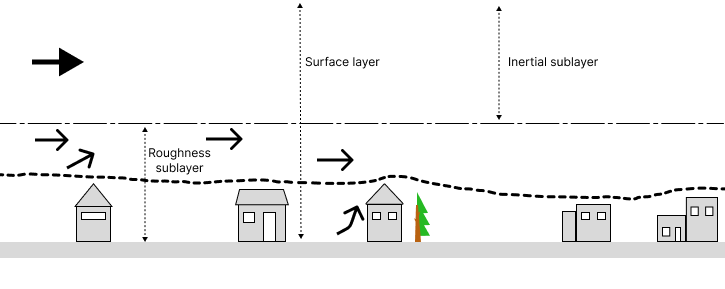
\includegraphics[width=\textwidth]{images/Localscale Boundary Layer.png}
    \caption{Microscale view of the urban climate, redrawn from~\cite{oke2006guideline}, (Todo)}
    \label{fig:microscale boundary layer}
\end{figure}

The microscale deals with the characteristics of each individual surface area. On of the main measurements on this layer is the surface temperature, which is primarily influenced by solar radiation. It is important to note, that surface and air temperatures are correlated, but this correlation varies greatly based on other surrounding influences such as wind velocity or humidity~\cite{stoll1992surface}.
todo: more\\
\\
Vertically UHIs can be devided into three mayor types~\cite{oke1976distinction, oke2017urban}, namely Boundary Layer Heat Island (BUHI), Canopy Urban Heat Island (CUHI) and Surface Urban Heat Islands (SUHI), that correspond with the boundary layer they can be monitored/measured in.
todo: more

\subsection{Canopy Urban Heat Island (CUHI)}

The canopy UHI is measured in the canopy boundary layer several meters above ground slightly below or on the average roof layer of the surrounding buildings, as seen in fig.~\ref{fig:microscale boundary layer}. The primary measurement in the canopy is air temperature, which is used to measure the urban heat island intensity (UHII)~\cite{oke1973city}, the most commonly used way of describing the heat island maginitude~\cite{kim2021urban}.\\
Since the beginning of modern climatology, mayor progress has been made in this research field, but methodologies and scientific rigor in CUHI research still seems to be lacking, as discussed by Stewart in 2011~\cite{stewart2011systematic}. Stewart found, that over 54\% of CUHI research was lacking proper methodologies or had other shortcommings such as a lack of site desciptions, where sensors were placed, or the disregard of non-urban factors such as local weather phenomena. In response, progress has been made in recent years by improving methodologies and ensuring correct measurements of climate-related data and study design and execution through various guidelines~\cite{oke2006guideline}, especially in urban settings, that require special care due to the huge amount of possible influences on local recording sites.\\

Todo: more

\subsection{Surface Urban Heat Island (SUHI)}

The surface temperature is measured directly at the surface of an object and is the main indicator of the surface urban heat island (SUHI). Surface temperature, in contrast to air temperature, typically is measured via remote sensing technologies like LST via satellites. Well-known satellites include MODIS, Landsat ... (todo list all), that all carry different types of instruments and sensors, that are able to take various measurements. Through the use of satellites, the spatial coverage is great, but raster sizes usually range from one kilometer to a hundred, so the spatial resolution is not that great compared to denser sensor networks. Additionally, these satellites are not geostionary to cover a wide range and therefore only take measurements during a handfull of times a day (todo: number of fly overs with example). Another downside is that satellites in many cases need clear-sky condidtions to measure surface temperature at ground level, as their sensors are not able to penetrate the cloud surface. As a solution, some technologies such as LIDAR (todo check if true) offer the approximation of the underlying surface temperature below clouds by measuring the out-going radiation of the surface.
todo: List of measurement types (microwaves etc.) with disadvantages\\
Surface and air temperatures can vary greatly, therefore a SUHI does not necessarily also imply a CUHI. Especially in extreme heat events, LST and air temperature can deviate greatly~\cite{good2016situ}.

\section{Smart Cities}

\subsection{Architecture Layers}

\subsubsection{Sensing Layer}

\subsubsection{Data Transportation Layer}

\subsubsection{Data Management Layer}

\subsubsection{Application Layer}

\subsection{Applications for ML-based Interpolation}
\subsubsection{UHI Detection in the Context of Smart Cities}

Smart Cities are `urban areas that exploit operational data [...] to optimze the operation of city services'~\cite{harrison2010foundations}, by collecting near-real-time data from physical and virtual sensors, integrating those data sources into an enterprise computing platform and performing complex analytics on them. With current urbanization trends (60\% ofd ppl living in cities 2060) and the ongoing global and urban warming (cite), research into smart cities has gotten a lot of attention recently (cite). On of the driving factors behind smart cities is next to progress in digitisation of cities the availibility of cheap smart sensors (cite), that enable a good spatiotemporal surveillance of factors in a smart city.\\
- goals and pillars
- architecture
- challenges

- classification of UHI detection into the smart city framework

In the context of UHI detection,

- testbeds, sensor networks (citizen owned)

- cross over to pollution detection

\section{Interpolation of Missing Data}

% First overview: interpolation techniques/history
% - foundation in statistics
% - adaptation for specific research areas (focus on temperature related research in this thesis)
%     - geostatistics (Krigin) -> probabilities need to be known
%         - climate research (macro) -> global warming, temperature trends
%         - urban climate research (micro) -> heat islands, polution
%     - ML approaches (deep learning, random forests etc.)
%         - list some approaches

In the context of urban environments, there are many measurements such as surface temperature, which are measured by sensors that have certain weaknesses. In the case of LST data collection, clouds play a mayor part and prevent surface temperature to be measured. In many LST data-sets (ref), measurements for cloud areas are simply defined as having no value. As many applications and algorithms need continous input data to work as expected, in this work we take a look on how interpolation, especially with the help of ML, can help solve this problem. In the context of LST data, this could mean interpolating the missing data either based on surrounding data (cite) or by integrating many different features such as air temperature, humidity, heat flux etc. in a ML model (cite).\\
- moving sensors for better spatial coverage into unobserved areas

\subsubsection{Interpolation vs. Extrapolation}

In this work, we focus on interpolation of missing data. Interpolation is the process of calculating/guessing missing values between given values. This could be a missing value in a time-series or a missing cell in a data grid (cite). In contrast, extrapolation is the prediction of values based on previous values, like predicting values based on historic time-series data, es in the case of weather forecasting. Due to time constraints, we only focus on the interpolation part, tho extrapolation could also play an important role in smart cities by predicting UHIs and warning citizens about potential future heat-related risks.

\subsection{Regression Analysis in Statistics}

Fundamentaly, regression analysis has its roots in mathematics, more specifically in the field of statistics.
todo: more

- foundation of other research fields, based in statistics/mathematics

- linear regression (least-squares)
- multiple regression models
- hierachical regression

- special cases
    - piecewise linear regression
    - inverse prediction
    - weighted least squares
    - logistic regression
    - poisson regression

\subsection{Interpolation in Geostatistics}

- spatiotemporal (kriging)
- time series prediction vs interpolation of missing data
- based on GIS 
- pipeline: fit measured data points to grid, interpolate missing squares
downside: cannot find local maximas/minimas

\subsection{Interpolation with Machine Learning Models}

% ML show promise in helping with interpolation tasks
% -> in order to train we need good data sets

- ML regression
